\chapter{高等数学：方程根与零点问题}

\section{方程根与零点问题}

\begin{problemblock}
\textbf{例1.} 函数 \(y=f(x)\) 的图像如图所示，在区间 \([a,b]\) 上可以找到 \(n(n\ge 2)\) 个不同的数
\[
x_1,x_2,\cdots,x_n,
\qquad
\frac{f(x_1)}{x_1}=\frac{f(x_2)}{x_2}=\cdots=\frac{f(x_n)}{x_n},
\]
则 \(n\) 的取值范围是（\quad）

A. \(\{3,4\}\)\qquad B. \(\{2,3,4\}\)\qquad
C. \(\{3,4,5\}\)\qquad D. \(\{2,3\}\)

\begin{center}
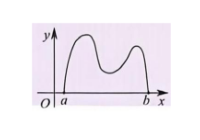
\includegraphics[width=.34\textwidth]{figures/gaoshu/page_028_graph.png}
\end{center}
\end{problemblock}
\begin{solutionblock}
\analysis{等式 \(\frac{f(x_i)}{x_i}\) 相同，几何意义是：从原点 \(O\) 作同一条直线 \(y=kx\)，它与曲线 \(y=f(x)\) 在 \([a,b]\) 上有 \(n\) 个交点。}
令
\[
g(x)=\frac{f(x)}x,\qquad x\in[a,b].
\]
则题目要求的是水平线 \(y=k\) 与函数 \(y=g(x)\) 的交点个数。

由图可知，原曲线在 \(a,b\) 两端落在 \(x\) 轴上，中间有两个峰和一个谷。相应地，斜率函数 \(g(x)=f(x)/x\) 从 \(0\) 开始，先上升到一个极大值，再下降到一个正的极小值，再上升到第二个极大值，最后下降到 \(0\)。因此：
\begin{itemize}
  \item 当水平线 \(y=k\) 位于两端 \(0\) 与中间极小值之间时，只与左右两段相交，得到 \(n=2\)；
  \item 当水平线经过中间极小值或第二个极大值等临界高度时，有一个交点由相切产生，得到 \(n=3\)；
  \item 当水平线位于中间极小值与较低的极大值之间时，四段都各交一次，得到 \(n=4\)。
\end{itemize}
同一条直线与这种图形最多只能穿过四个单调段，所以不可能得到 \(n=5\)。
\[
n\in\{2,3,4\}.
\]
\answer{B}
\method{方法二（斜率视角）}
把每个点 \(P(x,f(x))\) 对应为直线 \(OP\) 的斜率。沿曲线从 \(a\) 走到 \(b\)，斜率经历“升、降、升、降”四段变化，同一斜率最多在四段中各出现一次；通过选取普通高度和临界高度，分别得到 \(2,4,3\) 个点。
\examnote{这类图像题不要直接数 \(f(x)\) 的交点，而要把 \(\frac{f(x)}x\) 看成从原点到曲线上点的斜率。}
\end{solutionblock}

\begin{problemblock}
\textbf{例2.} 函数 \(f(x)\) 在 \([1,2]\) 上有二阶导数，\(f(2)=0\)，
\[
F(x)=(x-1)^2f(x),
\]
则 \(F''(x)\) 在 \((1,2)\) 上（\quad）

A. 没有零点 \qquad B. 必有零点 \qquad
C. 若有零点，必不止一个 \qquad D. 若有零点必唯一
\end{problemblock}
\begin{solutionblock}
\analysis{本题只给出端点信息，目标却是二阶导数零点，典型路线是连续两次使用 Rolle 定理。}
由
\[
F(x)=(x-1)^2f(x)
\]
可得
\[
F(1)=0,\qquad F'(x)=2(x-1)f(x)+(x-1)^2f'(x),
\]
故
\[
F'(1)=0.
\]
又因为 \(f(2)=0\)，所以
\[
F(2)=(2-1)^2f(2)=0.
\]
于是 \(F(1)=F(2)=0\)。由 Rolle 定理，存在 \(c\in(1,2)\)，使
\[
F'(c)=0.
\]
现在 \(F'\) 在 \([1,c]\) 上连续、在 \((1,c)\) 上可导，并且
\[
F'(1)=F'(c)=0.
\]
再次使用 Rolle 定理，存在 \(\xi\in(1,c)\subset(1,2)\)，使
\[
F''(\xi)=0.
\]
因此 \(F''(x)\) 在 \((1,2)\) 上必有零点。
\answer{B}
\examnote{端点重零点常常能多制造一次 Rolle 条件。本题的关键不是展开 \(F''\)，而是看出 \(F(1)=F(2)=0\) 且 \(F'(1)=0\)。}
\end{solutionblock}

\begin{problemblock}
\textbf{例3.} 讨论方程
\[
|x|^{1/4}+|x|^{1/2}-\cos x=0
\]
的根的个数。
\end{problemblock}
\begin{solutionblock}
\analysis{方程左端是偶函数，先在 \(x\ge0\) 上研究，再利用对称性。}
设
\[
\varphi(x)=x^{1/4}+x^{1/2}-\cos x,\qquad x\ge0.
\]
原方程左端为偶函数，所以正根成对出现。

先看区间范围。若 \(x\ge1\)，则
\[
x^{1/4}+x^{1/2}-\cos x\ge 1+1-1=1>0,
\]
故非负根只能出现在 \([0,1)\) 内。

又
\[
\varphi(0)=-1,\qquad \varphi(1)=2-\cos1>0,
\]
并且在 \(0<x<1\) 上
\[
\varphi'(x)=\frac14x^{-3/4}+\frac12x^{-1/2}+\sin x>0.
\]
所以 \(\varphi(x)\) 在 \((0,1)\) 上严格递增，由介值定理可知在 \((0,1)\) 内恰有一个正根。

由于原方程为偶方程，若正根为 \(\alpha\)，则 \(-\alpha\) 也是根；而 \(x=0\) 不是根。
\answer{共有 \(2\) 个实根。}
\method{方法二（单调值域法）}
令 \(t=|x|\)。方程等价于
\[
t^{1/4}+t^{1/2}=\cos x,\qquad t\ge0.
\]
右端不超过 \(1\)，左端当 \(t\ge1\) 时至少为 \(2\)，故只需看 \(0<t<1\)。在该区间左端函数随 \(t\) 增大而增大，而 \(\cos x\) 在 \(0<x<1\) 上递减，因此正半轴上至多一个交点，再结合端点异号得到恰有一个正根。
\examnote{含 \(|x|\) 且含 \(\cos x\) 的方程，先检查偶性和根所在范围，能大幅减少讨论。}
\end{solutionblock}

\begin{problemblock}
\textbf{例4.} 设 \(f(x)\) 在 \([0,+\infty)\) 上二阶可导，
\[
f(0)=0,\qquad f'(0)<0,\qquad f''(x)\ge M>0,
\]
则方程 \(f(x)=0\) 在 \((0,+\infty)\) 内不同实根的个数为（\quad）

A. \(3\) \qquad B. \(2\) \qquad C. \(1\) \qquad D. \(0\)
\end{problemblock}
\begin{solutionblock}
\analysis{条件 \(f''(x)\ge M>0\) 表示函数严格凸，并且 \(f'(x)\) 至少线性增大；\(f(0)=0,f'(0)<0\) 表示曲线从原点向下出发。}
由 \(f''(x)\ge M>0\)，对 \(x>0\) 积分得
\[
f'(x)\ge f'(0)+Mx.
\]
再积分得
\[
f(x)=f(0)+\int_0^x f'(t)\,dt
\ge f'(0)x+\frac{M}{2}x^2.
\]
当 \(x\to+\infty\) 时，右端趋于 \(+\infty\)，故 \(f(x)\to+\infty\) 的趋势足以保证存在充分大的 \(X\)，使 \(f(X)>0\)。

另一方面，由 \(f'(0)<0\)，当 \(x>0\) 充分小时有 \(f(x)<0\)。因此在某个小正数 \(\delta\) 处 \(f(\delta)<0\)，而充分大的 \(X\) 处 \(f(X)>0\)。由介值定理，\((\delta,X)\) 内至少有一个零点。

再证明至多一个。因为 \(f''(x)>0\)，\(f'(x)\) 严格递增，\(f\) 是严格凸函数。若 \((0,+\infty)\) 内有两个不同零点 \(\alpha<\beta\)，又 \(f(0)=0\)，则 \(f\) 在 \(0,\alpha,\beta\) 三点取零。由 Rolle 定理，存在
\[
\xi_1\in(0,\alpha),\qquad \xi_2\in(\alpha,\beta)
\]
使 \(f'(\xi_1)=f'(\xi_2)=0\)。再对 \(f'\) 用 Rolle 定理，存在 \(\eta\in(\xi_1,\xi_2)\)，使 \(f''(\eta)=0\)，这与 \(f''(x)\ge M>0\) 矛盾。

所以正半轴内恰有一个零点。
\answer{C}
\method{方法二（图像法）}
\(f''>0\) 说明曲线严格上凸，导数从负值开始并最终变为正值；函数先下降后上升。它从 \(f(0)=0\) 出发先到负值，最后升到正值，因此只能穿过 \(x\) 轴一次。
\examnote{根个数题要分“存在”和“唯一”。存在常用介值定理，唯一常用单调性、凸性或 Rolle 反证。}
\end{solutionblock}

\begin{problemblock}
\textbf{例5.} \(f(x)\) 在区间 \(I\) 上任意阶可导，且
\[
f^{(n)}(x)\ne0,
\]
证明方程 \(f(x)=0\) 在 \(I\) 上至多有 \(n\) 个根。
\end{problemblock}
\begin{solutionblock}
\analysis{这是 Rolle 定理的标准连用结论：函数零点太多，会迫使高阶导数出现零点。}
反证。若方程 \(f(x)=0\) 在 \(I\) 上至少有 \(n+1\) 个不同实根，记为
\[
x_0<x_1<\cdots<x_n.
\]
由于
\[
f(x_0)=f(x_1)=\cdots=f(x_n)=0,
\]
对每个区间 \((x_{i-1},x_i)\) 使用 Rolle 定理，可得 \(f'\) 至少有 \(n\) 个不同零点。

再对这些零点两两之间继续使用 Rolle 定理，可得 \(f''\) 至少有 \(n-1\) 个不同零点。如此重复，经过 \(n\) 次后得到：\(f^{(n)}\) 至少有 \(1\) 个零点。

这与题设 \(f^{(n)}(x)\ne0\) 矛盾。因此 \(f(x)=0\) 在 \(I\) 上至多有 \(n\) 个根。
\answer{已证：至多有 \(n\) 个根。}
\examnote{“第 \(n\) 阶导数不为零”常用来控制原函数根的上限；每用一次 Rolle，零点个数至少减少 1。}
\end{solutionblock}

\begin{problemblock}
\textbf{例6.} 证明：
\[
2^x-x^2-1=0
\]
恰有 \(3\) 个实根。
\end{problemblock}
\begin{solutionblock}
\analysis{先找出三个根存在的区间，再用高阶导数控制根的总数。}
设
\[
F(x)=2^x-x^2-1.
\]
显然
\[
F(0)=1-0-1=0,\qquad F(1)=2-1-1=0.
\]
又
\[
F(4)=16-16-1=-1<0,\qquad F(5)=32-25-1=6>0.
\]
由介值定理，在 \((4,5)\) 内至少有一个根。于是方程至少有三个实根：\(0,1\) 以及 \((4,5)\) 内的一个根。

下面证明至多三个。因为
\[
F'''(x)=(\ln2)^3 2^x>0,
\]
所以 \(F'''(x)\ne0\) 对一切实数成立。由例5的结论，\(F(x)=0\) 在 \(\mathbb R\) 上至多有 \(3\) 个实根。

综上，方程恰有 \(3\) 个实根。
\answer{恰有 \(3\) 个实根，其中两个为 \(0,1\)，另一个在 \((4,5)\) 内。}
\method{方法二（导数形态法）}
\[
F'(x)=(\ln2)2^x-2x,\qquad
F''(x)=(\ln2)^2 2^x-2,\qquad
F'''(x)>0.
\]
因此 \(F''\) 严格增，\(F'\) 至多有两个极值点，\(F\) 的零点总数不可能超过三个；再结合上面的三个变号位置，得到恰有三个根。
\examnote{指数函数减多项式的根个数题，常用“足够高阶导数符号固定”来给根数上界。}
\end{solutionblock}

\begin{problemblock}
\textbf{例7.} 求曲线
\[
y=e^{-x/2}
\]
与曲线
\[
y=x^3-3x
\]
的交点个数。
\end{problemblock}
\begin{solutionblock}
\analysis{交点个数就是方程 \(x^3-3x-e^{-x/2}=0\) 的根个数。先用变号找根，再用三阶导数控制上界。}
设
\[
H(x)=x^3-3x-e^{-x/2}.
\]
先找存在性：
\[
H(-2)=-8+6-e<0,\qquad
H(-1)=-1+3-e^{1/2}=2-\sqrt e>0,
\]
所以 \((-2,-1)\) 内有一个根；
\[
H(-1)>0,\qquad H(0)=-1<0,
\]
所以 \((-1,0)\) 内有一个根；
\[
H(\sqrt3)=3\sqrt3-3\sqrt3-e^{-\sqrt3/2}<0,\qquad
H(2)=8-6-e^{-1}=2-e^{-1}>0,
\]
所以 \((\sqrt3,2)\) 内有一个根。

下面证明至多三个。计算导数：
\[
H'(x)=3x^2-3+\frac12e^{-x/2},
\]
\[
H''(x)=6x-\frac14e^{-x/2},
\]
\[
H'''(x)=6+\frac18e^{-x/2}>0.
\]
由例5的思想，若 \(H\) 有四个或更多零点，则 \(H'''\) 必有零点，矛盾。因此 \(H\) 至多有三个零点。

所以两条曲线恰有三个交点。
\answer{交点个数为 \(3\)。}
\examnote{交点个数题先转为差函数零点个数。若已经能找出若干变号区间，再用 Rolle 或高阶导数给上界即可闭合证明。}
\end{solutionblock}

\begin{problemblock}
\textbf{例8.} 设方程
\[
\frac{\tan x}{x}=k
\]
在 \(\left(0,\frac{\pi}{4}\right)\) 内有实根，则常数 \(k\) 的取值范围为（\quad）

A. \(0<k<\frac4\pi-1\) \qquad
B. \(\frac4\pi-1<k<\frac4\pi\)

C. \(1<k<\frac4\pi\) \qquad
D. \(\frac4\pi-1<k<1\)
\end{problemblock}
\begin{solutionblock}
\analysis{这是函数值域定参题。只需求 \(\frac{\tan x}{x}\) 在开区间 \(\left(0,\frac\pi4\right)\) 上的值域。}
设
\[
\phi(x)=\frac{\tan x}{x},\qquad 0<x<\frac{\pi}{4}.
\]
则
\[
\phi'(x)=\frac{x\sec^2x-\tan x}{x^2}.
\]
令
\[
u(x)=x\sec^2x-\tan x,
\]
则
\[
u'(x)=\sec^2x+2x\sec^2x\tan x-\sec^2x
=2x\sec^2x\tan x>0.
\]
又 \(u(0^+)=0\)，故 \(u(x)>0\)，从而 \(\phi'(x)>0\)。因此 \(\phi\) 在 \(\left(0,\frac\pi4\right)\) 上严格递增。

端点极限为
\[
\lim_{x\to0^+}\frac{\tan x}{x}=1,
\qquad
\lim_{x\to(\pi/4)^-}\frac{\tan x}{x}=\frac{1}{\pi/4}=\frac4\pi.
\]
由于区间是开区间，端点值取不到，所以
\[
k\in\left(1,\frac4\pi\right).
\]
\answer{C}
\method{方法二（不等式法）}
在 \(0<x<\frac\pi4\) 上有 \(\tan x>x\)，故 \(\tan x/x>1\)。又 \(\tan x/x\) 严格递增，最大端点趋于 \(4/\pi\)，同样得到 \(1<k<4/\pi\)。
\examnote{“方程在区间内有根”常等价于“参数属于左端函数在该区间上的值域”。开区间端点极限通常不取等号。}
\end{solutionblock}

\begin{problemblock}
\textbf{例9.} 已知方程
\[
\frac1x-\frac{1}{e^x-1}=k
\]
在区间 \((-\infty,0)\) 内有实根，求常数 \(k\) 的取值范围。
\end{problemblock}
\begin{solutionblock}
\analysis{仍是值域定参题。负半轴上的式子不太直观，令 \(t=-x>0\) 可把区间转成正半轴。}
令 \(t=-x>0\)。则
\[
\frac1x-\frac{1}{e^x-1}
=-\frac1t-\frac{1}{e^{-t}-1}
=-\frac1t+\frac{1}{1-e^{-t}}.
\]
记
\[
\psi(t)=\frac{1}{1-e^{-t}}-\frac1t,\qquad t>0.
\]
先求端点极限。由
\[
e^{-t}=1-t+\frac{t^2}{2}+o(t^2),
\]
可得
\[
1-e^{-t}=t-\frac{t^2}{2}+o(t^2),
\]
因此
\[
\lim_{t\to0^+}\psi(t)=\frac12.
\]
又当 \(t\to+\infty\) 时，
\[
\frac{1}{1-e^{-t}}\to1,\qquad \frac1t\to0,
\]
故
\[
\lim_{t\to+\infty}\psi(t)=1.
\]

下面证明 \(\psi(t)\) 严格递增。计算
\[
\psi'(t)=-\frac{e^{-t}}{(1-e^{-t})^2}+\frac1{t^2}.
\]
于是 \(\psi'(t)>0\) 等价于
\[
(1-e^{-t})^2>t^2e^{-t}.
\]
两边同乘 \(e^t>0\)，等价于
\[
(e^{t/2}-e^{-t/2})^2>t^2,
\]
即
\[
2\sinh\frac t2>t.
\]
而 \(s>0\) 时 \(\sinh s>s\)，所以该不等式成立。因此 \(\psi\) 在 \((0,+\infty)\) 上严格递增。

故原式在 \((-\infty,0)\) 上的值域为
\[
\left(\frac12,1\right).
\]
\answer{\(\displaystyle \frac12<k<1\)。}
\method{方法二（级数主部加单调性）}
在 \(x\to0^-\) 时
\[
\frac1{e^x-1}=\frac1x-\frac12+O(x),
\]
所以原式趋于 \(1/2\)；在 \(x\to-\infty\) 时原式趋于 \(1\)。再由上面的导数判定得函数在负半轴上单调，故取值范围为 \((1/2,1)\)。
\examnote{遇到 \(e^x-1\) 的零点附近表达式，熟练使用 \(\frac1{e^x-1}=\frac1x-\frac12+O(x)\) 很省时间。}
\end{solutionblock}

\begin{problemblock}
\textbf{例10.} 
\begin{enumerate}[label=(\arabic*), leftmargin=2.2em]
\item 讨论
\[
F(x)=e^{-x}\left(1+x+\frac{x^2}{2!}+\cdots+\frac{x^n}{n!}\right)
\]
的单调性；
\item 讨论方程
\[
1+x+\frac{x^2}{2!}+\cdots+\frac{x^n}{n!}=0
\]
根的个数。
\end{enumerate}
\end{problemblock}
\begin{solutionblock}
\analysis{括号内是 \(e^x\) 的 \(n\) 阶 Taylor 多项式。乘上 \(e^{-x}\) 后求导会发生整齐抵消。}
记
\[
P_n(x)=1+x+\frac{x^2}{2!}+\cdots+\frac{x^n}{n!}.
\]
则
\[
P_n'(x)=1+x+\frac{x^2}{2!}+\cdots+\frac{x^{n-1}}{(n-1)!}=P_{n-1}(x).
\]
因此
\[
F'(x)=e^{-x}\bigl(P_n'(x)-P_n(x)\bigr)
=e^{-x}\bigl(P_{n-1}(x)-P_n(x)\bigr)
=-\frac{e^{-x}x^n}{n!}.
\]

因为 \(e^{-x}>0,n!>0\)，所以 \(F'(x)\) 的符号由 \(-x^n\) 决定：
\begin{itemize}
  \item 若 \(n\) 为奇数，则 \(x^n<0\) 当 \(x<0\)，\(x^n>0\) 当 \(x>0\)。故 \(F'(x)>0\) 在 \((-\infty,0)\) 上成立，\(F'(x)<0\) 在 \((0,+\infty)\) 上成立。于是 \(F\) 在 \((-\infty,0)\) 上单调增加，在 \((0,+\infty)\) 上单调减少；
  \item 若 \(n\) 为偶数，则 \(x^n\ge0\)，且除 \(x=0\) 外 \(x^n>0\)。故 \(F'(x)\le0\)，并且除 \(x=0\) 外严格为负，\(F\) 在 \(\mathbb R\) 上单调减少。
\end{itemize}

再讨论方程 \(P_n(x)=0\)。由于 \(e^{-x}>0\)，所以 \(P_n(x)=0\) 与 \(F(x)=0\) 等价。

若 \(n\) 为偶数，则
\[
\lim_{x\to-\infty}F(x)=+\infty,\qquad F(0)=1,\qquad \lim_{x\to+\infty}F(x)=0^+,
\]
且 \(F\) 单调减少，所以 \(F(x)>0\) 对一切 \(x\) 成立，方程无实根。

若 \(n\) 为奇数，则
\[
\lim_{x\to-\infty}F(x)=-\infty,\qquad F(0)=1.
\]
又 \(F\) 在 \((-\infty,0)\) 上单调增加，因此 \((-\infty,0)\) 内恰有一个零点；在 \((0,+\infty)\) 上 \(P_n(x)>0\)，故没有正根。

\answer{单调性：\(n\) 奇数时 \(F\) 在 \((-\infty,0)\) 增、在 \((0,+\infty)\) 减；\(n\) 偶数时 \(F\) 在 \(\mathbb R\) 上减。根的个数：\(n\) 奇数时恰有 \(1\) 个实根；\(n\) 偶数时无实根。}
\method{方法二（Taylor 余项法）}
由
\[
e^x=P_n(x)+\frac{e^\xi x^{n+1}}{(n+1)!}
\]
也可辅助判断 \(P_n\) 的符号趋势：正半轴上各项均正无根；负半轴上则由 \(F=e^{-x}P_n\) 的单调性判定奇偶情形。
\examnote{这题的核心抵消是 \(P_n'-P_n=-x^n/n!\)。计算到这一行，单调性和根数几乎同时解决。}
\end{solutionblock}
